\chapter{Metaheuristics}
\section{Introduction}
This chapter provides an insight into the workings of the various metaheuristics used in this research. We first define what we mean by the term \emph{metaheuristics} and then discuss each of the selected methods in turn.
Random Search, Hill Climbing, Simulated Annealing, Evolutionary Programming, Genetic Programming, Evolutionary Strategies and Genetic Algorithms are examined in detail, providing background on the origins of the method, a short summary of the algorithm, and finally, some discussion on the operators used and the selection methods employed

Metaheuristics are a class of approximate methods that are designed to attack hard combinatorial optimzation problems. They are often employed where classical heuristics have failed to be effective and efficient. Metaheuristics are computational procedures rather than computational algorithms\footnote{An Algorithm is a specific class of computational procedure that consists of a well-ordered collection of unambiguous and effectively computable operations that, when executed, produces a result and halts in a finite amount of time.}, typically exploring the solution landscape by starting from some randomly chosen point. They differ from heuristics and from formal computational algorithms in that they assume very little knowledge of the problem domain. They are what Artificial Intelligence has termed weak methods in that they are general strategies intended to be applicable to entire classes of problems. 

\section{Genetic Algorithm}
A Genetic Algorithm (GA)~\cite{holland}~\cite{goldberg} is a population-based method that simulates the evolution of individual structures through the process of selection, reproduction, recombination and mutation.
The GA models itself on the processes of evolution in nature by creating a population of individuals represented by chromosomes. These are, in essence, a set of character strings that are analogous to the chromosomes that we see in our own DNA. The individuals in this population evolve over the lifetime of the algorithm.

Crossover or recombination, which is the process of exchanging genetic information, happens in an environment where the probability of selection is a function of the fitness of the individual. Fitness in this context is a measure of the individuals success in solving the problem. Individuals which solve the problem are said to be perfectly fit, they have achieved the highest possible score on the task.
The fitness measure used to select individuals to undergo genetic operations such as crossover can range from simple fitness-proportionate selection to tournament-based selection where individuals in a subgroup compete and the fittest is selected. 
Mutation also plays a role in the GA process, while mutation may be random the process of the GA (as a simulation of a genetic process) itself is not a "random search" for a solution to a problem (highly fit individual). The GA uses stochastic processes, but the result is distinctly non-random.

\label{ga_operators}Previous analysis of GE~\cite{ieee2001} has used a Variable-Length GA as the means of directing the search. As in this previous analysis the experiments in this thesis use a steady-state population employing the standard GA operators of crossover and mutation.  The GA used in this research employs variable-length one point crossover with random mutation (see Figure~\ref{ga_operators_crossover})  operating at the bit-level level. Two non-standard operators, \label{sec:duplicate}\emph{Duplication} and \emph{Swapping}  (see Figure~\ref{ga_operators_dupswap})  which work at the codon level are also used. Duplication involves copying a sequence of genes of random length and placing them  between the last and second last gene, while the Swap operator does a positional swap of two randomly selected genes. 

The GA algorithm used in this research takes the following form: 

\begin{center}
\begin{enumerate}
\item Randomly create an initial population of \emph{n} solutions.
\item Calculate and normalise the fitness of the individuals through scaling.
\item Select two parents using roulette wheel selection mechanism.
\item Create two offspring from the selected parents by applying crossover, mutation, duplication and swap operations at set probabilities.
\item Replace the least fit individual in the population with the selected offspring if they have lower fitness than the selected offspring.
\item Go to step 3 until \emph{n} selections of offspring have been made.
\item Go to step 2 until the required solution has been found or the maximum generations have been reached. 
\end{enumerate}
\end{center}


\begin{figure}[]
\centerline{\hbox{
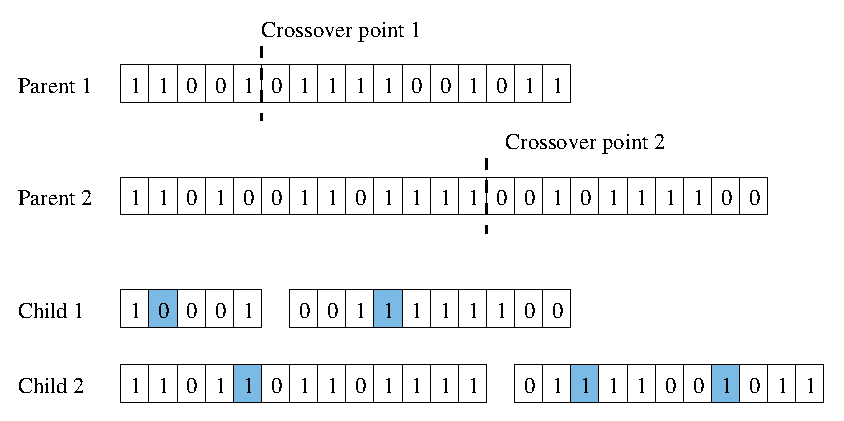
\psfig{file=Chapter3/graphs/ga_operators_crossover.ps,width=4in}}}
\caption[Crossover Operator with Mutation]{Crossover Operator with Mutation, used by GA. The figure shows the effects of the combined operators on selected genomes}
\label{ga_operators_crossover} 
\end{figure}

\begin{figure}[]
\centerline{\hbox{
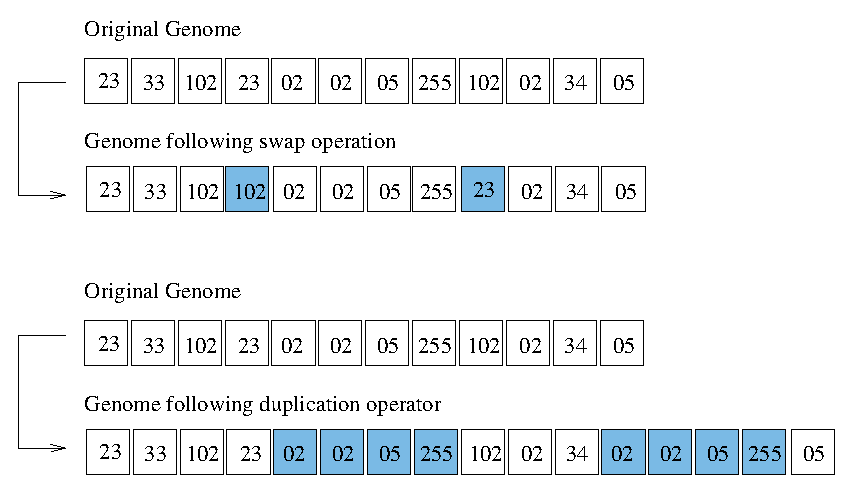
\psfig{file=Chapter3/graphs/ga_operators_duplicate.ps,width=3in}}}
\caption[Duplicate and Swap Operators]{Duplicate and Swap Operators, used by GA. The figure shows the effects of each operator on a selected genome}
\label{ga_operators_dupswap}
\end{figure}


\subsection{Ripple Crossover}
\label{ripple_crossover}Ripple Crossover~\cite{ripple} is a term used to describe the operation of crossover in GE. When a crossover point is selected in GE on a closed grammar (see Section~\ref{grammars}) all sub trees to the right of the crossover point are removed leaving an incomplete spine with multiple crossover points. For a context free grammar with multiple symbols the sub-trees removed do not have a constant interpretation, often causing radical re-interpretation of the codons involved. One of the consequences of ripple crossover is that on average half of the genetic material of an individual is exchanged during the crossover operation creating a global search throughout the course of a run. The disruptive nature of this global search mitigates against getting stuck in local optima by driving  improved fitness generation after generation. 


The grammar used in this example is:
\begin{verbatim}
E ::== X | Y | (+ E E) | (* E E) | (- E E) | (/ E E).
\end{verbatim}

\begin{figure}[]
\centerline{\hbox{
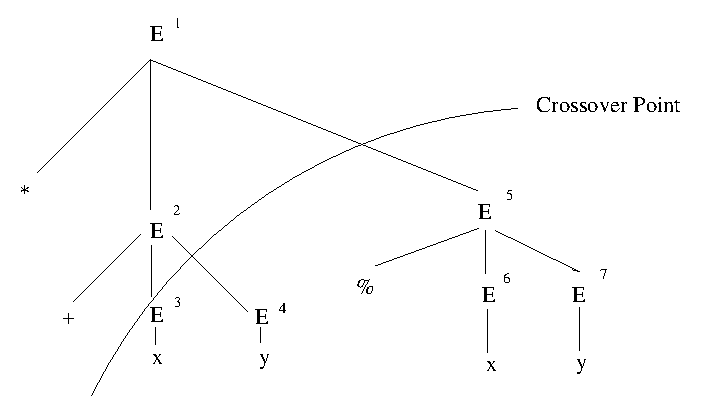
\psfig{file=Chapter3/graphs/ripple_xover.ps,width=3in}}}
\caption[Ripple Crossover Derivation Tree]{Ripple Crossover, Derivation Tree with Crossover site marked.}
\label{ripple1}
\end{figure}

Figure~\ref{ripple1} shows the effect of crossover on the derivation tree for a closed grammar. All sub-trees to the right of the crossover point are removed leaving a spine (shown in Figure~\ref{ripple2}) and a number of tails (shown in Figure~\ref{ripple3}). The removal of crossover point 3 has also resulted in the removal of crossover points 4, 5, 6 and 7, leaving an incomplete spine requiring 3 sub-trees to be complete. The removed tails, which are exchanged in the crossover operation, can then be used to complete crossover points in another tree. 




\begin{figure}[]
\centerline{\hbox{
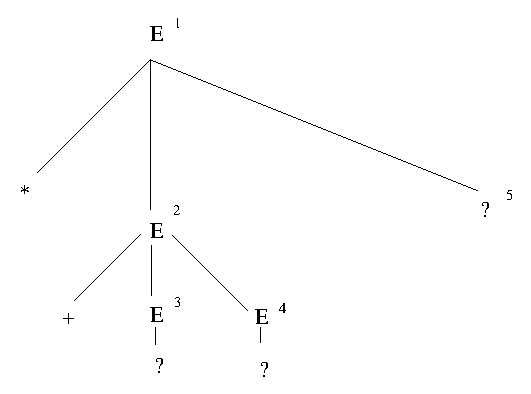
\psfig{file=Chapter3/graphs/ripple_xover2.ps,width=3in}}}
\caption{\label{ripple2}Ripple Crossover, Derivation Tree Spine after Crossover.}
\end{figure}



\begin{figure}[]
\centerline{\hbox{
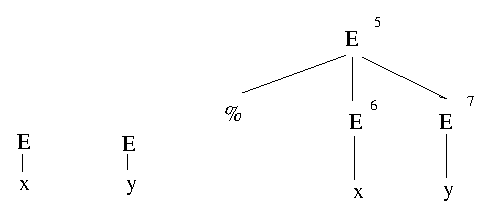
\psfig{file=Chapter3/graphs/ripple_xover3.ps,width=3in}}}
\caption{\label{ripple3}Ripple Crossover, Derivation Tree Tails after Crossover.}
\end{figure}


\section{Genetic Programming}
Genetic Programming (GP)~\cite{koza}~\cite{koza1}~\cite{koza2} is an Evolutionary Algorithm that evolves parse trees. Although it is not evaluated directly as part of this research it does provide a useful yardstick for performance on the problems evaluated in the trials detailed later. Much of the early analysis of GE~\cite{ieee2001} was presented as a comparative study against the efforts of GP on identical problems. 

Parse trees (see section~\ref{parse_trees}) can be used to represent programs in any language. These parse trees are evolved by GP using a combination of mutation and recombination. 

Closure, which is an important property in GP, exists when any terminal integer or variable can be passed to any function and any return type of a function can be passed as an argument to any other function. This ensures legal trees are maintained  as the parse trees change in the course of the evolution. However, this property also imposes the constraint that standard GP programs can only handle a single type. 

The programs in the population are composed of elements from the FUNCTION SET and the TERMINAL SET, which are typically fixed sets of symbols selected to be appropriate to the solution of problems in the domain of interest. An example of these is shown below.
\begin{verbatim}
GP function set F = {+,*,-,/}
Arity of functions  {2,2,2,2}
GP terminal set T = {X,Y}
\end{verbatim}

These are similar to the grammars shown in the previous section. The single non-terminal \emph{E} ensures closure.
In the Lisp programming language there is no distinction between the program and data, data objects can be manipulated as Lisp expressions, this feature, and its  ability to handle the linked data structures used in GP has made it a popular choice in the development and implementation of the method. However the method is easily accommodated in many  non-Lisp programming environments.
Recombination in GP involves taking  randomly selected sub trees in the individuals (selected according to fitness) and exchanging them.
The basic algorithm is as follows:

\begin{center}
\begin{enumerate}
\item Randomly create an initial population of random compositions of the functions and terminals of the problem (programs).
\item  Evaluate each program in the population and assign it a fitness value. 
\item Using fitness as the selection mechanism create a new population through mutation and recombination.
\item Go to step 2 until the required solution is found or the maximum evaluations have been reached. 
\end{enumerate}
\end{center}

\section{Random Search}
Random search cannot be strictly regarded as a metaheuristic, because it is essentially a random sampling of the search space. An initial solution is generated and its fitness calculated, then each new randomly generated solution is evaluated relative to the current one.  A new solution is accepted if its fitness is greater than that of the current solution. This process continues for a defined number of evaluations. The basic random search algorithm used for these trials is shown below.

\begin{center}
\begin{enumerate}
\item Randomly create an initial solution and determine its fitness. 
\item Randomly create a new solution and determine its fitness. 
\item Compute the change in fitness ($\delta F$) of the system between the two solutions. 
\item If $\delta F > 0 $ accept the new solution else reject the new solution and retain the current solution. 
\item Go to step 2 until the required solution is found or the maximum evaluations have been reached. 
\end{enumerate}
\end{center}

\section{Simulated Annealing}
The Simulated Annealing search technique is modeled on the way crystals form in solids during the cooling process. The quality of the crystals formed in the cooling process is dependent on the rate of cooling. The randomness provided by thermal energy allows atoms to escape from locally optimal configurations (meta-stable states) and form an optimum minimum energy crystalline structure.
\label{schedule}The rate of cooling is governed by an annealing schedule, which consists of an initial temperature, a rule for decrementing the temperature, a set number of iterations at a particular temperature and a final temperature.

The process and algorithms used in simulated annealing comes from the laws of thermodynamics which state that at a temperature $t$, the probability $P$ for a change  in energy of magnitude $\delta E$ is given by 

\large
\begin{displaymath}
P(\delta E) = e ^{ \frac{-\delta E}{kt}}
\end{displaymath}
\normalsize

\par\noindent where $k$ is the physical constant known as Boltzmann's constant. In a simulated version of annealing this equation is used within a system that is cooling toward a steady  state. 
For a general optimization problem, the temperature is just a parameter that governs the probability of increasing the cost function at any step. The usual Metropolis algorithm form~\cite{rosenbluth}  used  for general optimisation problems is 
\label{sa_algorithm}
\begin{center}
\begin{enumerate}
\item Select a starting temperature. 
\item Randomly create an initial solution and determine its fitness. 
\item Make a random trial change in the current solution. 
\item Compute the change in fitness ($\delta F$) of the system due to the trial change. 
\item If $\delta F > 0 $ accept the new solution else compute the acceptance probability $p = e^{\frac{-\delta C}{t}}$. 
\item Generate a random number $r$ in the interval [0,1]. 
\item Accept the new solution if $ p \ge r$ else  retain the current solution. 
\item Go to step 2 until the required solution has been found or the maximum evaluations have been reached.
\item Reduce the temperature, reset the evaluations counter to 0  and go to step 2 until the minimum temperature has been reached. 
\end{enumerate}
\end{center}

\par\noindent In simple terms the search technique permits the acceptance of dis-improving solutions with a probability which decreases as the process progresses and the temperature drops. The temperature must be decremented in sufficiently small steps, ensuring that the size of these steps has a logarithmic relationship with the number of iterations. A simple logarithmic cooling schedule is known to be optimal, allowing the temperature to be lowered at every iteration.


\section{Hill Climbing}
Hill Climbing is a simple but powerful metaheuristic. In its simplest form the search method attempts to find a global maximum by moving in an uphill direction. Random Mutation Hill-climbing (RMHC)~\cite{mitchell} uses random sampling of nearby points in the search space in order to determine the uphill direction. The Hill Climbing algorithm used in these experiments uses a similar approach, however mutation is carried out at the codon level. A noted shortcomings of Hill Climbing is the possibility that it will wander randomly through the search space when presented with plateaus in which all neighboring points have similar fitness values or that it will become trapped when it reaches a local minima/maxima. There are many variations on the basic algorithm, which attempt to address this weakness. One common variation is random-restart or multi-start hill climbing. Multi-start hill climbing~\cite{duvivier} generates a random starting solution and then hill-climbs to a local optimum. Once at a local optimum it repeats this process by generating a new random solution from which to hill-climb. The algorithm used in the various experiments, which is based on the simple form of Hill Climbing, is shown below:

\begin{center}
\begin{enumerate}
\item Randomly create an initial solution and determine its fitness. 
\item Make a random trial change in the current solution.  
\item Compute the change in fitness ($\delta F$) of the system between the two solutions. 
\item If $\delta F > 0 $ accept the new solution else reject the new solution and retain the current solution.
\item Go to step 2 until  the required solution has been found or the maximum evaluations have been reached. 
\end{enumerate}
\end{center}

\par\noindent Both the Hill Climbing and Simulated Annealing algorithms used in this study use a selection of four operators to explore the search space. The operators have been selected to allow subtle changes in the genomes by allowing a single mutation select alternate productions from the BNF grammar. The operators used  \emph{Force-up} and \emph{Force-down} (see Figure~\ref{operators_hcsa}) provide a means of selecting alternate productions by incrementing or decrementing a single randomly chosen codon. Two additional operators \emph{Grow} and \emph{Shrink} provide a means of expanding and contracting the genome into different areas of the search space. The Force-up and Force-down operators will always force the selection of a different production from the grammar, consequently \emph{neutral mutation} discussed in section~\ref{degeneracy} does not occur. The shrink operator removes the last codon from the genome while the grow operator adds a single codon whose value is randomly chosen.
One of the requirements of Simulated Annealing is that the applied mutations be probabilistically reversible, thus the probability of generating x from y needs to be equal to the probability of generating y from x. The implications of this are that the operator pairs Grow/Srink and Force-up/Force-down should have the same probability of occurrence.


\begin{figure}[]
\centerline{\hbox{
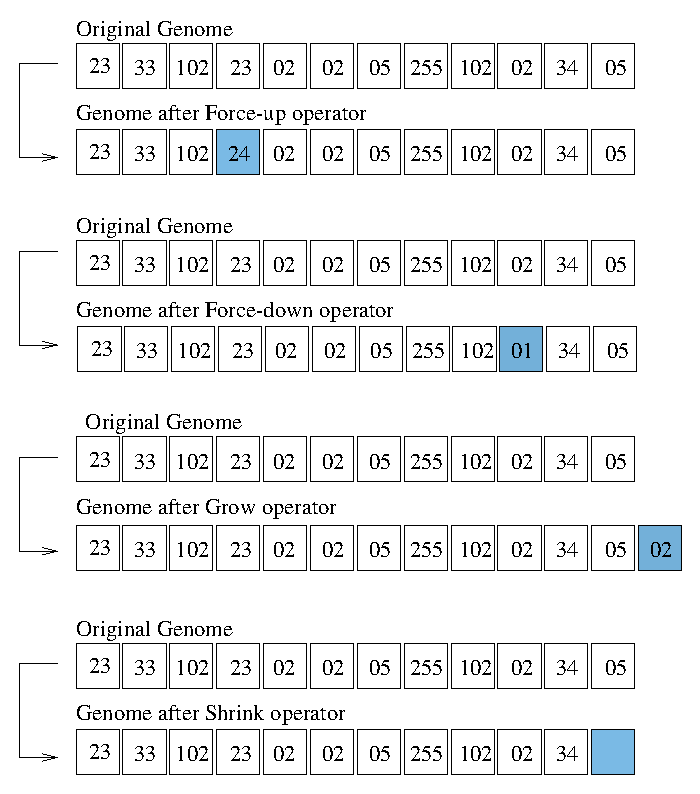
\psfig{file=Chapter3/graphs/operator.ps,width=4in}}}
\caption{ Operators, used by Hill Climbing and Simulated Annealing to explore the search space.}
\label{operators_hcsa}
\end{figure}

\section{Evolutionary Programming}
\label{ep}Evolutionary Programming (EP) had its origins in the work of Fogel, Owens and Walsh in the 1960s. It re-emerged in the 1980s when his son L.J.Fogel extended the approach to applications involving continuous parameter optimisation. Standard EP in its original form does not use any self-adaption mechanism, however Meta-EP which has many features in common with Evolutionary Strategies (see section ~\ref{es}), incorporating variances into the genotype. 
These variances evolve along with the object values. Unlike Evolutionary Strategies Meta-EP does not use a recombination or crossover operator. Each parent produces one offspring through mutation. In recent years EP like ES has been more strongly associated with continuous parameter optimisation, however applications of EP with some form of self-adaption has also featured in discrete optimisations~\cite{fogel}. Both the continuous and discrete forms are described  below.


\label{strategy_variables}The algorithm associated with the continuous form is shown below. In this context an individual or solution consists of a genome and one or more strategy variables. The mutation of the offspring includes the mutation of both the genome and the associated strategy variables.

\begin{center}
\begin{enumerate}
\item Randomly create an initial population of \emph{n} solutions.
\item Create \emph{n} offsprings by making a copy of this population.
\item Mutate the offsprings.
\item Combine the original population and the mutated offsprings.
\item Determine the fitness of each member of the combined population. 
\item Select the best \emph{n} individuals from the combined population.
\item Go to step 2 until the required solution has been found or the maximum generations  have been reached. 
\end{enumerate}
\end{center}

For continuous parameter optimisation using the meta-EP model mutation  proceeds as follows:
First the object variable is mutated as follows:
\begin{displaymath}
X_i^{'} = X_i + \sqrt{V_i}\cdot N(0,1)
\end{displaymath}


where \\
$X^{'}_i$ is the value of the mutated object variable at index i. \\
$X_i$ is the current value of the object variable at index i. \\
$\sqrt{V_i}$ is the square root of the variance at index i. \\
$N(0,1)$ is a normally distributed one-dimensional random variable having expectation zero and standard deviation 1. \\


The strategy variable (i.e variance) is the mutated as follows
\begin{displaymath}
V_i^{'} = V_i\cdot exp(\tau^{'}\cdot N(0,1) + \tau\cdot N_i(0,1))
\end{displaymath}


where \\
$V^{'}_i$ is the value of the mutated variance at index i. \\
$V_i$ is the current value of the variance at index i. \\
$\tau^{'}$ is commonly proportional to$ (\sqrt{2n})^{-1}$, where n is the number of dimensions in the object variable.  \\
$\tau$ is commonly proportional to $(\sqrt{2\sqrt{n}})^{-1}$, again n is the number of dimensions in the object variable. \\
$N(0,1)$ is a normally distributed one-dimensional random variable having expectation zero and standard deviation 1. \\
$N_i(0,1)$ is as above but the variable is sampled anew for each value of i. \\

 
\label{ep_selection}Selection in EP consists of pair wise comparison over the union of parents and offspring ($2\mu$ individuals). Each individual is compared to \emph{q} randomly chosen opponents. The number of wins for the individual in each of these tournaments is recorded. The top $\mu$ individuals with the highest number of wins go forward to form the next generation.

Traditional approaches to discrete optimisation~\cite{fogel} involves using a uniform random distribution to select one of a number of mutation operators. Discrete optimization with self-adaption builds on this approach by incorporating a probability mass function into the individual. The probability mass function determines the extent of the mutation. This probability mass function  evolves by perturbing the parents probability using a Gaussian random vector with zero mean and an arbitrarily chosen variance. The perturbed probabilities are scaled using a scaling factor so that the sum of all probabilities is one. 

To facilitate self-adaption each individual in the population consists of a genome and a number of strategy variables which  evolve with the genome through successive generations. A strategy variable can influence the genome in any number of ways, for example, the rate of mutation to be applied to the genome could evolve as a strategy variable rather than being a fixed quantity as in the case of a Genetic Algorithm. Another example would  be the use of a strategy variable to determine where in the genome string the mutation will take place. 

The process of generating the offspring consists of first copying an individual (genome and strategy variable), then randomly perturbing the strategy variables and finally using the strategy variables to mutate the genome. The algorithm for self-adaptive discrete optimisation is given below.


\begin{center}
\begin{enumerate}
\item Randomly create an initial population of \emph{n} solutions.
\item Randomly create the initial strategy variables for each member of the population. 
\item Create \emph{n} offsprings by making a copy of the population and its associated strategy variables.
\item Mutate the strategy variables using a Gaussian random vector.
\item Mutate the offsprings using the mutated strategy variables.
\item Combine the original population and the mutated offsprings.
\item Determine the fitness of each member of the combined population. 
\item Select the best \emph{n} individuals from the combined population.
\item Go to step 3 until the required solution has been found or the maximum generations  have been reached. 
\end{enumerate}
\end{center}



\section{Evolutionary Strategies}
\label{es}Evolutionary Strategies (ES) emerged from the joint development of Bienert, Rechenberg and Schwefel in the 1960s at the Technical University of Berlin. Two principal forms of the strategy emerged, the $(\mu + \lambda)-ES$ strategy (elitist strategy) allows the best $\mu$ individuals from the union of parents ($\mu$) and offspring ($\lambda$) to survive while the ($\mu,\lambda$) strategy allows the best ($\mu$) offspring's survive to the next generation. A significant part of ES is the capability for self-adaption, this is achieved by allowing the strategy variables evolve along with the object variables.

An individual in ES consists of an object variable vector (x) and optional strategy variables consisting of a number of standard deviations $(\sigma)$ and a number of rotation angles $(\alpha)$. Parents produce offspring by applying normally distributed mutations, these mutations control the step size, which in turn determines the mutability of the object variables.

Learning takes place at two levels, both in the optimisiation of the objective variables and the strategy variables. The strategy variables represent the standard deviation of a ($0,\sigma_i$) Gaussian distribution with an expectancy value of 0. With this the parents should produce offsprings similar to themselves on average.
Mutation can involve all three elements of the individual, the object variable vector, the standard deviations and the rotation angles. The mutation of the standard deviation strategy variables involves a multiplicative, logarithmic normally distributed process as follows:
 
The mutation of the standard deviations proceeds as follows:

\begin{displaymath}
\sigma_i^{'} = \sigma\cdot exp(\tau^{'}\cdot N(0,1) + \tau\cdot N_i(0,1))
\end{displaymath}

where \\
$\sigma_i^{'}$ is the resulting mutated value of the standard deviation. \\
$\sigma_i$ is the current value of the standard deviation. \\
$\tau$ is a factor suggested by Schwefel to be set $\propto (\sqrt{2\sqrt{n}})^{-1}$ where n is the number of dimensions in the object variable. \\
$\tau^{'}$ is suggested by Schwefel to be set to $\propto (\sqrt{2n})^{-1}$. \\
$N(0,1)$ is a normally distributed one-dimensional random variable having expectation zero and standard deviation 1. \\
$N_i(0,1)$ is as above but the variable is sampled anew for each value of i. \\


The mutation of the rotation angle  proceeds as follows:

\begin{displaymath}
\alpha_j^{'} =  \alpha_j + \beta\cdot N_j(0,1)
\end{displaymath}
where
$\alpha_j^{'}$ is the resulting mutated value of the rotation angle. \\
$\alpha_j$ is the current value of the rotation angle. \\
$\beta$ is a constant recommended by Schwefel to be set at $\approx 0.0873$. \\
$N_j(0,1)$ is a is a normally distributed one-dimensional random variable having expectation zero and standard deviation 1 which is sampled anew for each value of j. \\


The mutation of the object variable vector is as follows:
\begin{displaymath}
\vec{x}^{'} = \vec{x} + \vec{N}(\vec{0},C(\vec{\sigma}^{'},\vec{\alpha}^{'}))
\end{displaymath}
where
$\vec{x}^{'}$ is the resulting mutated object variable vector. \\
$\vec{x}$ is the current object variable vector. \\
$C(\vec{\sigma}^{'},\vec{\alpha}^{'})$ is a covariance matrix of standard deviations $\vec{\sigma}^{'}$ and rotation angles $\vec{\alpha}^{'}$. \\
$\vec{N}(\vec{0},C(\vec{\sigma}^{'},\vec{\alpha}^{'})$ is a normally distributed random variable having expectation zero and standard deviation $C(\vec{\sigma}^{'},\vec{\alpha}^{'})$. \\

For the case where rotation angles are not used the formula reduces to:

\begin{displaymath}
\sigma_i^{'} = \sigma\cdot exp(\tau^{'}\cdot N(0,1) + \tau\cdot N_i(0,1))
\end{displaymath}
\begin{displaymath}
\vec{x}^{'} = \vec{x} + \sigma_i^{'} \cdot N_i(0,1)
\end{displaymath}


\label{es_recombination}A significant difference between ES and EP (see Section~\ref{ep}) is the use of recombination. A number of different crossover or recombination strategies are used in ES. Schwefel recommends discrete recombination on object variables and panmictic intermediate recombination on strategy parameters. 

Discrete recombination (see Figure~\ref{discrete_recombination} ) involves selecting two parents at random from the population and creating an offspring, which consists of object variables genes drawn with equal probability from both parents. More formally: 

\begin{displaymath}
X^{'}_i = X_{S,i} or X_{T,i} 
\end{displaymath}

where \\
$X^{'}_i$ is the value of the offsprings object variable at index i. \\
$X_{S,i}$ is the value of the first randomly selected parent at index i. \\
\emph{or} in this context indicates that either parent can be selected with equal probability. \\
$X_{T,i}$ is the value of the second randomly selected parent at index i. \\


Panmictic (global) intermediate recombination  (see Figure~\ref{intermediate_recombination}) involves selecting one parent at random from the population and creating an offspring through recombination with other randomly selected parents. These other parents are chosen randomly for each instance of the index i, again formally stated: \\

\begin{displaymath}
X^{'}_i = 0.5 \times (X_{S,i} + X_{T_i,i}) 
\end{displaymath}

where \\
$X^{'}_i$ is the value of the offsprings object variable at index i. \\
$X_{S,i}$ is the value of the first randomly selected parent at index i. \\
$X_{T_i,i}$ is the value of another randomly selected parent at index i. A different parent is randomly selected anew for each value of the index i. \\

\label{es_selection_strategies}There are two preferred methods of selection used in ES as indicated above. The $(\mu + \lambda)-ES$ strategy allows the best $\mu$ individuals from the union of parents ($\mu$) and offspring ($\lambda$) to survive while the ($\mu,\lambda$) strategy allows the best ($\mu$) offspring's survive to the next generation. The  ($\mu,\lambda$) strategy which limits individuals to one generation is generally preferred ~\cite{back}.

The ratio $\mu/\lambda$ determines the convergence property of the evolutionary strategy. Decreasing $\mu$ leads to path orientated search (predictive or exploratory methods providing fast local convergence) while increasing $\mu$ leads to a volume orientated search (assumes the whole feasible region must be scanned which increasing chances of finding a global optimum)~\cite{back} pages 46-47. The logarithmic normal distribution for the variations of standard deviations insures that smaller modifications must occur more often than larger ones. 


\begin{figure}[]
\centerline{\hbox{
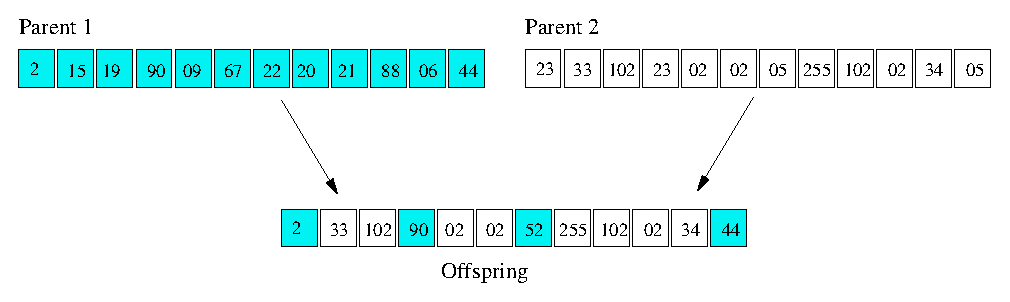
\psfig{file=Chapter3/graphs/discrete_recombination.ps,width=4in}}}
\caption[Discrete Recombination]{Discrete Recombination, the offspring is formed by codons from either parent with equal probability of selection.}
\label{discrete_recombination}
\end{figure}



\begin{figure}[]
\centerline{\hbox{
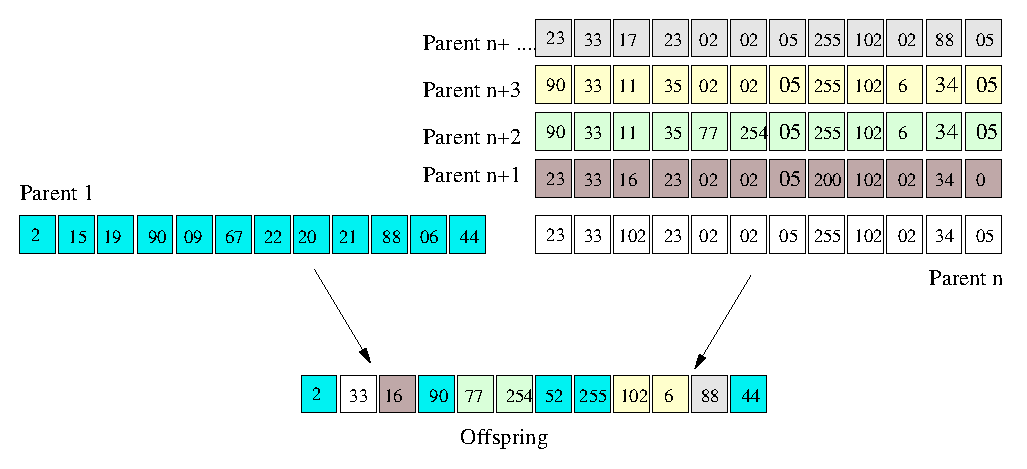
\psfig{file=Chapter3/graphs/intermediate_recombination.ps,width=4in}}}
\caption[Intermediate Recombination]{Intermediate Recombination, the offspring is formed by codons from a selected parent and n other randomly (equal probability of selection) selected parents.}
\label{intermediate_recombination}
\end{figure}

\subsection{Relationship between EP and ES}

ES like EP has primarily been associated with optimisation of continuous data. Optimisation of discrete data can be achieved by using a uniform random distribution to select one of a number of mutation operators. As with EP, an element of self-adaption can be introduced by incorporating a probability mass function into the individual. The probability mass function which determines the extent of the mutation  evolves by perturbing the parents probability using a Gaussian random vector with zero mean and an arbitrarily chosen variance. The perturbed probabilities are scaled using a scaling factor so that the sum of all probabilities are one. 

\subsection{Self Adaptive Discrete Optimisation}
Each individual in the population consists of a genome and a single strategy variable. This strategy variable determines the rate of mutation to be applied to the genome. The strategy variable which  evolves along with the genome, consists of an integer value that corresponds to the number of codons altered during mutation,
The process of generating the offspring involves copying an individual (genome and strategy variable), then randomly perturbing the strategy variable and finally using the strategy variable to determine the rate of mutation to be applied to the genome. The algorithm for self-adaptive discrete optimisation which is the form of EP used in these experiments is given below.


\begin{center}
\begin{enumerate}
\item Randomly create an initial population of \emph{n} solutions.
\item Randomly create an initial strategy variable for each member of the population. 
\item Using selected recombination method create \emph{2n} offsprings.
\item Mutate the strategy variable using a Gaussian random vector.
\item Mutate the offsprings using the mutated strategy variables.
\item Determine the fitness of each member of the combined population. 
\item Select the best \emph{n} offspring to replace the parent population.
\item Go to step 3 until the required solution has been found or the maximum generations  have been reached. 
\end{enumerate}
\end{center}



\section{Summary}
In this chapter we have introduced each of the selected metaheuristics. Genetic Algorithms, Genetic Programming, Evolutionary Programming and Evolutionary Strategies are population-based methods that evolve populations of solutions using a combination of selection, mutation and recombination, while Simulated Annealing and Hill Climbing are local search techniques that explore the search space by modifying a single individual. Random search is, in essence, a sampling of the search space, providing a useful indication of the density of solutions and accordingly the relative difficulty of problems. In our examination of these techniques we have presented the basic algorithm involved and discussed the operators and selection strategies that charachterise each method.











